\documentclass[11pt]{article}

\usepackage[a5paper,left=2cm,right=1cm,top=1cm, bottom=1.5cm]{geometry}
\usepackage{array}
\usepackage{makecell}
\usepackage[all]{nowidow}
\usepackage{wrapfig}
\usepackage{enumitem}
\usepackage{multicol}

\usepackage{hyperref}
\hypersetup{
    colorlinks=true,
    urlcolor=sokolblue,
    }

\usepackage[czech]{babel}
\usepackage[utf8]{inputenc} 
\usepackage{ellipsis}

\usepackage{fontspec}
\newfontfamily{\tyrs}{Sokol Tyrs}
\newfontfamily{\fugner}{Sokol Fugner}

% \usepackage{lmodern}
% \usepackage[T1]{fontenc} 
\usepackage{anyfontsize}
\newcommand{\titlesize}{\fontsize{56pt}{67pt}}


\usepackage[dvipsnames]{xcolor}
\definecolor{sokolred}{RGB}{228, 5, 33}
\definecolor{sokoldarkred}{RGB}{200, 0, 30}
\definecolor{sokolblue}{RGB}{45, 46, 135}

\usepackage{tikz}
\usetikzlibrary{calc}

\usepackage{fancyhdr}

\fancypagestyle{standard}{%
    \fancyhf{}
    \fancyhead[LO]{%
        \begin{tikzpicture}[overlay,remember picture]
            \fill [color=sokolred] (current page.north west) rectangle ($ (current page.south west) + (1cm,0cm) $);
            \fill [color=sokolred] ($ (current page.north west) + (1.1cm,0cm) $) rectangle ($ (current page.south west) + (1.2cm,0cm) $);
        \end{tikzpicture}
        }
    % \fancyhead[RE]{%
    %     \begin{tikzpicture}[overlay,remember picture]
    %         \fill [color=orange](current page.north east) rectangle
    %             ($ (current page.south east) + (-1cm,0cm) $);
    %     \end{tikzpicture}
    %     }
    \fancyfoot[C]{%
      \begin{tikzpicture}[overlay,remember picture]
        \fill [color=sokolred] ($ (current page.south east) + (-1.5cm,1.3cm) $) rectangle ($ (current page.south east) + (0cm,0.5cm) $)
         node [pos=0.5,color=white] {\large\tyrs{\thepage}\hspace*{0.5cm}};
      \end{tikzpicture}
    }

    \renewcommand{\headrulewidth}{0pt}
    \renewcommand{\footrulewidth}{0pt}
}



\fancypagestyle{uvodnik}{%
    \fancyhf{}
    \fancyfoot[C]{%
      \begin{tikzpicture}[overlay,remember picture]
        \fill [color=sokolred] ($ (current page.south east) + (-1.5cm,1.3cm) $) rectangle ($ (current page.south east) + (0cm,0.5cm) $)
         node [pos=0.5,color=white] {\large\tyrs{\thepage}\hspace*{0.5cm}};
      \end{tikzpicture}
    }

    \renewcommand{\headrulewidth}{0pt}
    \renewcommand{\footrulewidth}{0pt}
}

\fancypagestyle{blank}{%
    \fancyhf{}
    \fancyfoot[C]{}

    \renewcommand{\headrulewidth}{0pt}
    \renewcommand{\footrulewidth}{0pt}
}


\newcommand{\post}[1]{%
\begin{center}
{\huge \tyrs #1}
\end{center}
}

\newcommand{\subpost}[1]{%
\vspace*{12pt}
\begin{center}
{\Large \tyrs #1}
\end{center}}

\newcommand{\signature}[2]{%
  \begin{flushright}
    \textbf{#1}\\#2
  \end{flushright}
}

\newcommand{\luv}{\clqq\kern-0.07em}
\newcommand{\ruv}{\kern0.07em\crqq\kern0.1em}

\usepackage{csquotes}
\DeclareQuoteAlias{german}{czech}
\MakeOuterQuote{"}

\usepackage[normalem]{ulem}


\begin{document}

%% title
\newgeometry{margin=1cm}
\pagecolor{sokolred}
\color{white}
\pagenumbering{gobble}
\begin{center}

\vspace*{\fill}

\includegraphics*[width=0.75\textwidth]{logo-140-vert-white.pdf}

{\titlesize \fugner ZPRÁVY}

{\titlesize \tyrs SOKOLA LIBEŇ}

\vspace*{1cm}

{\large ročník L · číslo 2 · červen 2024}

\vspace*{\fill}
\end{center}

\clearpage
\normalcolor
\nopagecolor
\pagenumbering{arabic}

%% úvodník
\pagestyle{uvodnik}
\newgeometry{margin=1.5cm}


{\fontsize{48pt}{57pt} \fugner \color{sokolred} \noindent Úvodník}
\hfill
{\textbf{náčelník}} %\raisebox{24pt}{...}


\vspace*{12pt}

Zas šest let a je tu slet. Blíží se nám největší sláva, jakou my sokolové máme!

240 Libeňáků posledního půl roku poctivě nacvičuje na XVII. všesokolský slet.
Co to vlastně znamená?

Deset z~dvanácti skladeb si jednotliví cvičitelé nastudovali a předali svým cvičencům. Trpělivě vyčkali na úbory, vyměnili a doučili nové cvičence za ty, kteří se nakonec sletu nebudou moci zúčastnit. Dozjistili si detaily skladeb a průběžně mění choreografie podle finálních počtů na sletišti v~Edenu.

Cvičenci vyvinuli snahu v~závislosti na své skladbě. Ti nejmenší prokázali šikovnost a odvahu, ti v~bouřlivém věku potlačili počáteční absenci nadšení a vzdor, jenž k~jejich věku patří, ženy napřely úsilí k~nacvičení opravdu těžkých skladeb, muži se naopak přiučili skromnosti.

Na oblastním sletu v~Brandýse nad Labem, který funguje jako generálka k~všesokolskému sletu, bylo na našich cvičencích vidět, že mají nacvičeno dobře. Ne že by snad vystoupení byla ideální, sem tam se ještě mezi značkou ztratíme, ale celkový dojem je dobrý a ve srovnání s~ostatními jednotami jsme na tom opravdu dobře.

V~první veliké slávě se ukážeme ve sletovém průvodu. To už do Prahy dorazí sokolové z~celého světa. Bude to první z~mnoha příležitostí v~celém týdnu potkat nové přátele, poznat bratry a sestry odjinud, prožít si spousty malých příběhů s~přáteli starými. Uvidíme veterány plakat dojetím, pocítíme radost a sounáležitost a hlavně se budem cítit jako sokolové spolu a jednotní.

Letošní slet má heslo Slet spojuje. Vzpomínám, jak jsem se při posledním XVI. sletu nachomýtnul k~sokolům z~Kanady a Švýcarska, kteří spolu secvičovali skladbu Princezna republika. Kolik lidí jsem na posledním sletu potkal, se kterými jsem od té doby pořád v~kontaktu a jak jsem se na ploše cítil. Slet nás spojí už tím, že spolu něco hezkého prožijeme. Ale budeme-li toto heslo mít v~průběhu sletového týdne pořád na mysli, můžeme mu jít naproti a uvést ho v~život. Byl bych rád, kdybychom našeho největšího svátku využili k~tomu, abychom se nesdružili a nestmelili jen v~našich cvičebních celcích a v~naší jednotě, ale abychom se skamarádili. Abychom poznali, co a jak cvičí jinde, abychom získali zkušenost a předali tu naši. A~nakonec jako jedna z~významných pražských jednot máme tu milou povinnost u~nás doma přivítat spoustu sester a bratrů, kteří v~Praze byli jen několikrát nebo dokonce nikdy. Buďme k~nim proto laskaví, pohostinní a přátelští, aby naši Prahu měli i za svou a cítili se tu dobře a jako doma.

Chovám ohromnou úctu ke všem autorům sletových skladeb. Děkuji všem cvičitelům a jejich pomahatelům za nacvičení skladeb v~rekordním počtu. Věřím všem Libeňákům, že nám v~celém sletovém týdnu a během skladeb budou dělat to nejlepší jméno svým chováním a precizností cvičení a těším se víc než na cokoli jiného.

\vspace*{\baselineskip}
\noindent
Na zdar našemu sletu!


\clearpage

%% termínka

\pagecolor{sokolred}
\color{white}
\renewcommand{\arraystretch}{1.2}

\newcommand{\boxheight}{14.5cm}

% \vspace*{\fill}
\post{TERMÍNOVÁ LISTINA AKCÍ JEDNOTY}
\vspace*{-20pt}

\begin{center}
\begin{tikzpicture}
  \draw [ultra thick,color=white](0.3cm,0cm) rectangle (12.3cm,\boxheight);
  \fill [color=white] (0cm,0.3cm) rectangle (12cm,\boxheight + 0.3cm)
  node [pos=.5, color=black] {
    \begin{tabular}{l  p{6.5cm}}
      21.–23. 6. (pá–ne) & příprava tábora (Velhartice)\\
      27. 6. (čt) & poslední cvičení žáků \\
      30. 6. (ne) & Sletový průvod \\
      4. a 5. 7. (čt, pá) & programy hromadných skladeb XVII.~všesokolského sletu \\
      5. 7. 2024 & zakončovací táborák\newline termín vyklizení skříněk \\
      6.–13. 7. & letní pobyt  pro předškolní děti a mladší školní děti (Janské Lázně) \\
      13.–20. a 20.–27. 7. & Pobyty rodičů a dětí (Janské Lázně) \\
      19.–21. 7. & dostavba tábora (Velhartice, pomocníci vítáni, informace u~vedoucích TO) \\
      19.–27. 7. & Letní tábor bývalých členů Jilmu (Velhartice) \\
      27. 7. – 10. 8. & Letní tábor Káňat (Velhartice) \\
      10. 8. – 1. 9. & Letní tábor Jilmu a Veverek (Velhartice) \\
      30. 8. – 1. 9. & bourání tábora (Velhartice, pomocníci vítáni, informace u~vedoucích TO)\\
      2. 9. (út) & zahájení cvičení žákyň, Rodičů a dětí a Předškolních dětí \\
      3. 9. (út) & zahájení cvičení žáků \\
      19. 9. (čt) & 24. ročník Běhu strmého \\
      28. 9. (so) & Noc sokoloven \\
      listopad & Oslavy 140. výročí založení Sokola Libeň \\
    \end{tabular}
  };
  %  node [color=black] {FOOBAR};
\end{tikzpicture}

\renewcommand{\arraystretch}{1}

\vspace*{12pt}
Sledujte naše stránky a zprávy ze systému EOS, kde budeme postupně uveřejňovat podrobnosti k~jednotlivým akcím.

\end{center}
\vspace*{\fill}

\clearpage
\nopagecolor
\normalcolor

%% normální obsah
\restoregeometry
\pagestyle{standard}

\post{Informace od starosty}

\subpost{Provoz v~šatnách a jejich úprava o~prázdninách}
Od pondělí 19. února jsou v~provozu zrekonstruované šatny. Už jsme našli nějaké nedostatky, ale postupně je odstraňujeme. Lépe jsme zajistili dveře klecí proti vypadnutí z~kolejniček, před šatnami přibyly dvě nástěnky na plakátky (aby se tyto nemuseli lepenkou lepit na čerstvě opravené dveře), máme naplánovanou výrobu laviček před sprchy, aby kryly boční hranu schodu, již je připravena montáž větracích mřížek do šatnových skříněk, aby v~nich lépe vysychaly vlhké věci (trička, cvičební obuv, ručníky) – bude se dělat během prázdnin – \textbf{majitele skříněk tedy prosíme o~jejich vyklizení nejpozději 5.7. večer}. Jinak jsme rádi, že se dodržuje čistý provoz v~šatnách (i když při chození dětských oddílů ven je to trochu nekomfortní – zout, dát si věci do klece a zase obout. Ale už jsme si zvykli).

Jedna prosba k~botníkům. Pokud si nechci boty zamykat, použiju poličku, pokud ano použiju malý zamykací šuplík a zamknu ho. Větší šuplíky jsou určené pro dětské oddíly, kdy se tam vejde více párů bot. Tak nám je neobsazujte vaším jedním párem – děkujeme. Prázdné šuplíky nechávejte odemčené a klíčky vracejte na háček. Mimochodem, nemá někdo doma klíček od botníku s~číslem 41 nebo 63. ty už nám nějaký týden chybí. 

Hlavním přínosem čistého provozu v~šatnách by měla být i větší čistota v~sálech. \textbf{Zásada, na které budeme stále striktně trvat je, že žádné venkovní boty nepřekročí práh šaten, a to ani v~ruce!} Prozatímní provozní řád nových šaten vám přišel z~EOSu a je umístěn i na našich internetových stránkách.

\subpost{Informace o~financích jednoty a o~zvýšení příspěvků}
Po zaplacení faktur za šatny nám v~lednu na účtu nezbylo z~původních 10,5 milionu ani 500 tisíc. Zatím nějak vycházíme. Byly peníze z~příspěvků za I. pololetí, něco přichází od nájemců nebytových prostor a taky už jsme byli podepsat smlouvu na grant z~Magistrátu (518 000,- na provoz sokolovny). Peníze dnes dorazily na účet, a tak bychom měli vyjít do září, kdy nám do pokladny zase přibude částka z~příspěvků na II. pololetí. Kromě toho máme informaci, že nám Praha 8 přisoudila cca 700 000,- z~grantu na sport dětí. A~také by měla něco dodat Národní sportovní agentura a nájemci za 3. čtvrtletí.

I~tak ale výbor rozhodl a \textbf{navýšení příspěvků od září v~jednotné výši o~200,- Kč na pololetí} (s~třemi drobnými výjimkami - turistické oddíly, senioři a senioři nad 80 let, kde je zvýšení nižší). V~ruku v~ruce s~tím jde i zvýšení nájmu školám, nesokolským oddílům i zvýšení režijních poplatků menších sokolských oddílů, a to o~cca 10\%. Již, v~lednu byly zvýšeny nájmy nebytových prostor taktéž o~10\%.

\subpost{Stavební práce v~sokolovně a kolem ní}
Byla opravena střecha severní malé terasy, kde zatékalo.

V~brzké době budeme muset opravit nízkou zídku z~kyklopského zdiva pod plotem hřiště gymnázia, kde vypadává spárovací omítka i celé kameny.

Před pár dny praskla v~noci na WC v~klubovně turistických oddílů hadička k~nádržce. Byla tak vyplavena klubovna, něco zateklo i do kotelny a v~přízemí za dámskými šatnami byl slušný bazén. Trochu to odnesla i nová výmalba stropu nad zadním schodištěm. Naštěstí se voda nedostala do sálu na parkety. Škody jsou tak naštěstí minimální. \textbf{Děkujeme panu vrátnému Přibylovi a uklízečce Ivě Duchačové za rychlé zvládnutí oné záplavy.}

V~létě nás kromě drobných úprav v~šatnách čeká i dovybavení nové podzemní místnosti, kompletní dostěhování věcí z~plechové garáže a pak i demontáž oné staré garáže. Na podzimní brigádě pak rozbití a odvezení starého betonu, úprava povrchu a zatravnění. 

Máme již projekt na propojení staré matriky s~nájemcem ABA Strategie. Čekáme na závazné stanovisko památkářů a pak se bude žádat o~stavební povolení. Rádi bychom toto propojení zrealizovali v~srpnu, aby se od září tyto prostory daly pronajmout (do února sloužily jako provizorní šatna).

Snad posledním problémem je řešení problému s~kolaudací podzemní místnosti, kde došlo k~nějakému šumu v~dokumentaci a obdržení negativního stanoviska od památkářů ke kolaudaci. V~závazném stanovisku památkářů se píše, že se vydává na základě předložené projektové dokumentace ke stavebnímu řízení, a tak i bylo vydáno stavební povolení, které jsme od architektů měli objednáno na klíč. Na památkářích je však zaevidováno toto povolení na studii, která předcházela projektu a stavba tam vypadá odlišně. Takže bylo vydáno ono negativní stanovisko. 

Architekti uznali svoje pochybení, na památkáře bylo zaslána žádost o~stanovisko k~projektu, kde jsou nějaké podmínky – třeba jiný vzhled vnějších stěn místnosti a zídky. Architekti nyní řeší, zda se na to pochybení vztahuje jejich pojistka. Momentálně stejně nemáme na předělání finance a stavebně se nejspíše bude řešit až v~roce 2025. Pak by snad už mohla být místnost zkolaudována.

\subpost{Nové vedení České obce sokolské}
Mimochodem, asi jste zaznamenali kauzy bývalé starostky ČOS a její asistentky. Novým starostou ČOS byl následně zvolen Martin Chlumský (Čedok), což jak jistě řada z~vás ví, je dlouholetý člen (asi 35 let) naší jednoty a bývalý jilmák. Tak mu držme palce, ať vede Sokol správnou cestou.

\subpost{Valná hromada}
Ve středu 20. 3. 2024 se konala Valná hromada Sokola Libeň. K~18. 3. měla naše jednota 821 členů (174 předškolních dětí, 140 žáků, 131 žákyň, 164 mužů a 212 žen), které na Valné hromadě zastupovalo 32 delegátů z~41 zvolených. Na Valné hromadě byla schválena výroční zpráva za rok 2023, zpráva kontrolní komise a rozpočet jednoty na rok 2024. Dále se probraly věci cvičební i k~provozu sokolovny za rok 2023 a přednesl se výhled činnosti na rok 2024. Valná hromada též vzala na vědomí změnu na místě náčelnice, tuto funkci opustila Alena Krásová a bude ji vykonávat Tomáš Dragoun.

\signature{Jiří Novák (Jirkan)}{starosta\\tel.: 602 284 198}

\vspace*{24pt}

\post{Jaro v~oddíle žáků a dorostenců}
Od posledních Zpráv, které vyšly koncem února, jsme se ve cvičení ani nezastavili. Bylo tolik dění, že dokonce vznikaly třenice mezi čtvrtečními oddíly (kdy v~jeden čas cvičí žáci i žákyně) o~prostor pro nácvik na akademii, na závody, na slet a pro běžné cvičení. Nakonec se to nějak zvládlo a výsledky snažení snad stály za to. A~teď tedy postupně o~tom jarním ruchu. Letošní docházka je zatím velmi početná. Nejnižší průměr od září 2023 byl v~lednu – rovných 50. Nejvyšší byl v~únoru – 65,4, kdy 20 kluků nemělo jedinou vynechávku. Každý měsíc je zapsáno přes 100 žáků. Průměry jsou skoro o~10 vyšší než v~předchozích letech. Tak ať nám to vydrží i v~dalším cvičebním roce. Trvá celoroční soutěž O~nejvěrnější docházku s~pravidelným každoměsíčním vyhlašováním a rozdáváním diplomků za 100\% docházku a také Zimní soutěž žáků v~počtu shybů na jeden zátah.

Cvičení venku s~atletickými disciplínami začalo 30. dubna a za dobrého počasí bude pokračovat do konce června. V~případě velké zimy nebo deště cvičíme v~sokolovně. I~ven se nosí jako úbor bílé tričko se znakem a modré trenky a vhodná sportovní obuv – žádné tepláky a bundy nejsou při cvičení potřeba, dostatečně se zahřejeme pohybem. \textbf{Začátek i konec hodiny je v~šatně!}  

\textbf{Poslední cvičení} před prázdninami bude ve \textbf{čtvrtek 27. června}, kdy proběhne i vyhlášení Zimní soutěže a Celoroční docházky. Kluci, přijďte všichni.

\subpost{Závody}
I~přes pilné nácviky na slet jsme nevypustili každoroční Závody všestrannosti v~gymnastice, atletice a plavání. 20 a 22. 2. 2024 se konaly Nominační závody žáků u~nás v~sokole. Gymnastické sestavy na kruzích, hrazdě, bradlech, přeskok, prostná a šplh si zkusilo 92 kluků (48 mladších žáků, 35 starších žáků a 8 dorostenců) a z~nich jsme vybrali 30 kluků (12 mladších, 14 starších a 4 dorostence) pro další nácvik na dubnové Závody všestrannosti.

Celopražské Závody všestrannosti proběhly o~víkendu 19.–21. 4. 2024. Vyslali jsme 11 mladších žáků, 9 starších žáků, 3 dorostence a 7 mužů. Celkem tedy 30 cvičenců. A~protože se v~žácích účastnilo celkem 31 závodníků z~naší župy, měli kluci jen 11 soupeřů a možnost mnoha dobrých umístění. V~jednotlivých disciplínách (plavání, gymnastika, šplh a atletika) jsme získali 23 medailových umístění. V~celém čtyřboji byl vítězem ve své kategorii M. Osoha. Kromě toho M. Cakl a V. Böhm brali 2. místa, H. Höschl 3., L. Bednář, O. Nekvapil, J. Šefrna a Š. Novák 4. místa.

Na celostátní finále všestrannosti postoupili z~mladšího žactva M. Osoha a M. Cakl, ze staršího žactva pak V. Böhm a H. Höschl.

Kromě závodníků jsme museli na závody samozřejmě vyslat i doprovázející cvičitele a rozhodčí – celkem to bylo 11 cvičitelů.

Celostátní finále všestrannosti mladšího žactva se konalo o~víkendu 25.–26. května v~Pardubicích. V~mladší kategorii se M. Cakl umístil na 15. místě mezi 22 soupeři (8. v~plavání a šplhu) a M. Osoha na 17. místě celkově (4. v~plavání a 7. v~atletice).

Kromě Závodů všestrannosti se ve středu 8. května se konal také gymnastický závod Praha Open (společný pražský závod pro Sokol a Českou asociaci Sport pro všechny), kam ze Závodu všestrannosti postoupilo 12 našich žáků. Deset se jich závodu zúčastnilo a vedlo si obdobně jako na župních závodech. Kromě toho závodili do výsledků všestrannosti i 3 muži.

Dva starší žáci a 3 muži nás budou o~víkendu 31. 5. – 2. 6. reprezentovat na celostátním Přeboru všestrannosti staršího žactva, dorostu a dospělých v~Praze, ale to je po uzávěrce zpráv.

\signature{Jiří Novák (Jirkan)}{}


\vspace*{24pt}

\post{Zpráva místonáčelníka}

\subpost{Akademie}
2. 3. 2024 se konala z~podzimu přeložená Tělocvičná akademie. Dopoledne 22 úderníků během 90 minut vyklidilo sál, přerovnalo nářadí, nanosilo a smontovalo pódia, umístilo 200 židlí, lavičky pro sezení cvičenců, namontovalo osvětlení a ozvučení a už mohly začít generálky některých skladeb. Před akademií si zájemci mohli prohlédnout nově zrekonstruované šatny, které byly pro běžný provoz otevřeny 19. února. Úderem 16. hodiny se pak před asi 300 diváky během 80 minut předvedlo 11 vystoupení, kterým předcházel slavnostní nástup v~krojích a historických cvičebních úborech s~prapory a slavnostní zahájení akademie.

Jako první zacvičilo 14 párů rodičů a dětí, následovala ukázka sletové skladby Babí léto, kde s~deštníky zacvičilo 8 žen, které na ploše vystřídalo 32 nezbedů a 4 dospělí z~oddílu předškoláků. Následovala opičí dráha v~podání 23 mladších žáků, které jistilo 9 cvičitelů, a po nich na plochu naskákalo se švihadly 14 děvčat z~oddílu Skipping Buddies, které sledovali 2 trenéři. Další ochutnávkou sletu bylo cvičení staršího žactva (12 kluků, 12 holek), které předvedlo ukázku skladby Fitness. Pěkné cvičení na lavičkách s~obručemi nacvičilo 27 mladších žákyň pod vedením 5 cvičitelek. Starší žáci (20) předvedli rozmanité přeskoky přes bednu a stůl, starší žákyně (16) pak předvedly své cviky na airtracku. Poslední ukázku sletu pak předvedlo 21 mladších žáků (a 3 doplňující cvičitelé) se skladbou Sokolhraní. Vrcholem a posledním číslem akademie bylo cvičení mužů (13) na bradlech zakončené vyzvednutím bradel nad hlavu i s~cvičencem.

Všechna cvičení se líbila a byla oceňována bouřlivým potleskem. A~pak rychle vše uklidit na svá místa. Zvládli jsme to za neuvěřitelných 35 minut. Díky všem cvičitelům, cvičencům i divákům a samozřejmě našemu obslužnému personálu (moderátor, zvukaři, osvětlovači, technická četa, fotografové) z~řad cvičitelstva.  

\subpost{Šibřinky}
V~sobotu 23. 3. 2024 byly na programu tradiční Šibřinky. Ráno se vše připravilo. Vyklidil se sál, přerovnalo nářadí, nanosily stoly a židle, pódia pro kapelu, nainstalovala se rozsáhlá výzdoba sálu, připravil se bar, skříně se sklenicemi, zapojil dřez pro mytí nádobí a provedly se další drobné práce. Přišlo 25 pomocníků, kterým vše trvalo 1,5 hodiny. Pak rychle na oběd a v~15:00 začaly Dětské šibřinky ve stylu Pata a Mata, na které dorazilo asi 90 dětí v~maskách.

Na programu byly tanečky, masky, vystoupení Skipping Buddies a v~druhé části pak bylo připraveno 10 soutěží inspirovaných příhodami dvou výše zmíněných nemotorů, po nichž byli úspěšní účastníci obdarováni drobnou odměnou. Díky všem 42 pomocníkům, kteří se postarali o~hladký průběh akce.

Okolo páté odpolední byly děti odeslány domů, aby rodiče a další zájemci mohli o~sedmé večerní dorazit na Šibřinky pro dospělé s~podtitulem Sletu zdar! Byla živá kapela, tombola, soutěž masek, občerstvení, předtančení, ukázka akrojógy, tři společné hromadné akce (tanec, taneční cvičení s~obručemi a nacvičení kousku staré sletové skladby Výlet s~aerobikem). Bylo asi 130 účastníků, kteří se dobře bavili až do druhé ranní. V~neděli pak 15 vytrvalců mezi 10. a 14. vše uklidilo. Děkujeme všem 27 pomocníkům, kteří drželi na večerních šibřinkách služby (snos a mytí nádobí, prodej občerstvení, obsluha na baru, točení piva). Zvláště pak děkujeme starším sestrám, které napekly spoustu výborných dobrot pro děti i pro dospělé.

\subpost{Brigády}
V~neděli 3. března proběhla Jarní brigáda v~sokolovně a okolí. Ruku k~dílu přiložilo 13 cvičitelů, 3 cvičitelky, 1 žák, 9 Jilmáků, 5 Veverek a 5 mužů. Celkem tedy 36 lidí.

Venku se natíral dřevěný plůtek, hrabalo listí na trávníku, připravovalo doskočiště, hrabalo listí před kostelem a zametal chodník před sokolovnou a nad doskočištěm. V~sokolovně se pak vzorně uklidila dílna a klubovna, umyla se okna na zadním schodišti po stavbě šaten, očistily se vršky vchodových zádveří, umylo se zábradlí a světla na vstupním schodišti, napasovaly se staré lavičky do haly, natřely se dveře pod zadním schodištěm na straně mužů, parním čističem se vydrhly sprchy, do šaten se namontovala zrcadla, na galerii se smontovaly a umístily botníky pro turistické oddíly, staré plechové zelené odpadkové koše se natřely na černo, aby ladily se šatnami, zrušily se dočasné šatny v~přízemí a do kočárkárny se vrátilo atletické vybavení, uklidilo se před nářaďovnou Srncova sálu i samotná nářaďovna, opět se zatěsnily zadní dveře, otřel prach v~nových šatnách ve větších výškách, demontovalo se zaslepení větracích mříží v~sále a proběhly i další drobné a úklidové práce.

Celkem to bylo asi 160 člověkohodin práce. Všem zúčastněným moc děkujeme. 
\clearpage
\vspace*{-36pt}
\subpost{Výlety}
V~sobotu 13. 4. se 89 Libeňáků sešlo na 66. Jarním Výletě Libeňského Sokola. Spolu s~jednotami ze Starého Města, Kobylis a Zlíchova jsme byli účastníky 57. srazu v~přírodě pražských žup. Vlakem jsme vyrazili z~Vysočan do Kojetic a pěšky pak po zelené k~jezírku V~lomu, kde proběhla Modrá stuha. Díky letošnímu teplému počasí už byla voda vyhřátá na 16,5 °C. Po nástupu s~Písničkou, Jazykohrátkami a Pamatovačkou jsme se přesunuli kousek do lesa na hru Džungle a po ní jsme kolem kostela a zámku v~Lobkovicích došli na místo srazu – louku na břehu Labe. Následoval oběd (s~Vařením pokrmu z~mléka) a pak už byla na programu hlavní věc dnešního dne – župní kolo Zálesáckého závodu zdatnosti (ZZZ). Účastnilo se 11 trojic žactva a 4 trojice dorostu. Nejprve byla mimo okruh disciplína oheň, pak se běžel okruh s~9 stanovišti (hvězdy, morseovka, uzlování, překážky, šošonský běh, hody na cíl, topografie, přírodniny, pamětihodnosti) a po doběhu ještě zdravověda a práce s~nožem. V~žactvu vyhrál Jilm před Starým Městem a další trojicí Jilmu a v~dorostu zvítězil Jilm před Veverkami a Starým Městem. Na celostátní finále postupují vždy první dvě trojice. V~mezidobí proběhl i miniZZZ pro menší děti. Pak už nástup s~vyhlášením výsledků obou závodů, rozdání Pamětních lístečků, volba data Podzimního srazu (12. 10.) a rychle do Neratovic na vlak. Byla to vydařená sobota s~vydařeným počasím.

O~víkendu 10.–12. května se konalo celostátní finále ZZZ v~Úpici. Ve starším žactvu se utkalo 20 trojic a Libeňská \textbf{trojka z~oddílů Jilm a Veverky vybojovala úžasné 2. místo}! V~dorostu bylo 13 trojic a naše hlídka obsadila 6. místo.

\subpost{Dětský den}
Ve čtvrtek 30. května se konal Dětský den. Po deštivém dopoledni přestalo v~půl třetí pršet a padlo rozhodnutí jít ven. Rychle se vše naložilo na vozík, který se odtlačil do parku, a za necelou hodinku začal s~malým zpožděním v~16:25 další Dětský den Sokola Libeň. Bylo připraveno 29 stanovišť a projížďky na kánoích (zde poprvé v~historii došlo k~nedobrovolnému koupání, a to hned dvakrát – poprvé převrátil kánoi rychle nastupující tatínek a podruhé nedočkavé dítě, které nedbalo pokynu, že nemá vystupovat – omlouváme se, ale lodivodi za to naštěstí nemohli).

Dorazilo 160 dětí, které si vesměs stihly obejít všechna stanoviště. V~18:30 byl konec soutěží, rozdání zbylých odměn a pak už plocha patřila na půl hodiny 12 šermířům. Dle ohlasu dětí i rodičů se odpoledne nadmíru vydařilo. Aby tomu tak bylo, muselo ruku k~dílu přiložit 53 pořadatelů (12 cvičitelů, 6 cvičitelek, 20 žáků, 8 žákyň, 5 mužů, 2 hosté) – všem moc děkujeme. 

Po skončení akce zase vše sesbírat, naložit, odvést, roznosit na svá místa v~sokolovně. A~pak si konečně na chvíli sednout na židli na trávníku u~doskočiště a dát si něco na grilu. A~ráno do práce. To je život cvičitele.

\subpost{Přípravy na slet}
V~neděli 14. 4. proběhl druhý secvik Sokolhraní, kdy chyběl pouze jeden omluvený žák – bylo to užitečné odpoledne. Kluci se konečně sešli všichni a viděli celou skladbu jako celek.

V~sobotu 11. 5. byl poslední (třetí) secvik Sokolhraní, na kterém jsme již kluky otáčeli do různých směrů a vzali je i ven na trávu, aby se oprostili od záchytných bodů v~tělocvičně a zvykli si cvičit kdekoli. 

O~víkendu 25.–26. května se v~Brandýse nad Labem konal oblastní slet. Celkem cvičilo skoro 2 300 cvičenců. V~pátek se i za naší účasti dělala příprava cvičiště včetně umístění cca 500 značek. Celou sobotu probíhaly zkoušky většiny skladeb. V~neděli ráno zbyly už jen zkoušky skladeb nejmenších dětí a od 11 hodin pak generálka. Okolo druhé vyšel od cvičiště sletový průvod k~místní sokolovně, soše T. G. Masaryka a do zámeckého parku s~pomníkem obětí světových válek. Ve tři odpoledne pak započal vlastní slet.

Zahájil jej slavnostní nástup s~prapory, proslovy, dekorování praporů sletovou stuhou a následně začala cvičit Věrná garda skladbu Jdi za štěstím. A~v~tu chvíli přišel i vydatný déšť trvající celou jejich desetiminutovou skladbu. Sklidili bouřlivý potlesk. A~pak už na promáčenou plochu nastupovaly další skladby už i s~naší účastí. Celkem nás z~Libně cvičilo 236. Čarodějky – mladší žákyně 23, V~rytmu srdce – ženy 32, Mravenci – předškoláci 31 dětí + 5 dospělých, Čmeláčci – rodiče a děti 16 párů, Rocková symfonie – ženy a muži 1, Sokolhraní – mladší žáci 24, S~tebou mě baví svět – rodinná skladba 0, Fitness – starší žactvo: 24 kluků, 18 holek, Babí léto – ženy 8, Leporelo – ženy 20, Před kamerou – muži 34. Na konci sletu ještě na rozloučenou Krokovka. V~publiku nechyběl starosta ČOS br. Martin Chlumský (mimochodem z~naší jednoty) a také hejtmanka Středočeského kraje Petra Pecková.

Těšit nás může, že jsme všechny skladby zacvičili moc pěkně (žáci předvedli zatím určitě nejlepší provedení) a taky, že slet v~Edenu je ještě před námi a nemusíme se ho bát, ale můžeme se na něj těšit. Díky i všem rodičům, že všech 48 žáků mohlo přijet, a těm, co se byli podívat osobně, že vydrželi přes počáteční nepřízeň počasí až do konce.   

\subpost{Na co se těšíme? Na slet!}
\begin{itemize}[
  itemsep=-3pt,
  leftmargin=2em,
  itemindent=-1em
]
  \item[] 30. 6. Sletový průvod půjde po trase Václavské náměstí, Národní třída, nábřeží, Rudolfinum, Pařížská, Staroměstské náměstí. Cvičenci jdou v~průvodu, příznivci jim mohou mávat na chodnících po trase.
  \item[] 2. 7. Sokol gala – ukázka špičkových sportovních výkonů v~O2 aréně. Pouze pro sletové cvičence, kteří projevili zájem.
  \item[] 1.–4. 7. Zkoušky jednotlivých skladeb v~Edenu
  \item[] 4. 7. večer od 21 hodin – První sletové vystoupení
  \item[] 5. 7. odpoledne od 14 hodin – Druhé sletové vystoupení
Pokud nemáte lístky přímo do Edenu, nemusíte zoufat, na ČT poběží přímý přenos.
  \item[] 5. 7. večer od cca 18–19 (až se stihneme přesunout z~Edenu k~sokolovně) bude Posletový táborák. Tam si všichni sdělíme dojmy z~právě skončeného sletu, možná bude konečně chvilka blíže se seznámit se spolucvičenci a taky možná dojde na malou upomínku na slet. Tak ať se u~táboráku sejdeme všichni jako na ploše při cvičení.
\end{itemize}

Sokolským prostorem se šíří zvěst, že ČOS dostala grant i na sletové úbory, a že by tedy mohly být zadarmo stejně jako sletové náčiní (nebo alespoň levnější). Pokud by to tak bylo, cvičenci by si platili pouze sletový průkaz. V~okamžiku, kdy se zpráva potvrdí, výbor rozhodne a bude vypsána platba pro sletové cvičence.

Mnoho radosti a optimismu do nadcházejícího léta přeje

\signature{Jiří Novák (Jirkan)}{místonáčelník\\tel.: 602 284 198}

\post{Turistický oddíl JILM a Veverky}
Už se blíží konec školního roku a s~ním i prázdniny a tábor, na který zavítáme opět k~Velharticím. Zatím pokračujeme v~nezměněném programu i počtu.

\vspace*{12pt}\noindent
Co jsme zažili:
\begin{itemize}[
  itemsep=-3pt,
  leftmargin=2em,
  itemindent=-1em
]
  \item[] 3. 3. (ne) pomohlo 14 našich členů na jarní brigádě při úklidu klubovny, dílny, na dvoře a všude, kde bylo potřeba.
  \item[] 16.–17. 3. (so–ne) jsme se vypravili na Aprílovou výpravu do jižních Čech, podívat se na naše nové tábořiště, které se velice zalíbilo, a těšíme se, až tam pojedeme na tábor. Cestou jsme se kochali krajinou podhůří Novohradských hor, navštívili zříceninu hradu Sokolčí a vylezli na rozhlednu.
  \item[] 3. 4. (st) proběhl tradiční Mistr signalizace, kdy mezi 17 kamarády zvítězila Opička.
  \item[] 13.–14. 4. (so–ne) jsme pořádali JVLS, sraz pražského trojžupí a semifinále ZZZ. K~Lobkovicím se vypravilo 19 našich členů, kteří se také zúčastnili ZZZ, kde v~žactvu zvítězili Štěpán, Shark a Alpík a na 3. místě se umístili Sojka, Manitou a Vilda, v~dorostu zvítězili Padák, Vinnetou a Hrom a 2. místě skončily Nina, Maruška a Bára. Výlet jsme si protáhli i na neděli, kdy jsme se šli z~Brandýsa nad Labem do Lysé nad Labem.
  \item[] 17. 4. (st) se uskutečnil Mistr uzlování, kdy se mezi 19 kamarády prouzlovala na první místo Opička.
  \item[] 10.–12. 5. (pá–ne) se konal přebor v~Zálesáckém závodu zdatnosti v~Úpici v~kempu Radeč, kam přišlo poměřit své dovednosti a znalosti osm našich členů. Hlídka žactva (Štěpán, Shark a Alpík) vybojovala 2. místo mezi 20 soupeři, Opička jako náhradník v~dorostenecké hlídce Tišnova na 2. místě a hlídka dorostu (Maruška, Nina a Bára) se umístila na 6. místě ze 13.
\end{itemize}

\vspace*{6pt}
\noindent
Co nás čeká:
\begin{itemize}[
  itemsep=-3pt,
  leftmargin=2em,
  itemindent=-1em
]
  \item[] 31. 5. – 2. 6. (so–ne) Boj družin – místo loďovky, z~důvodu nedostatku zkušených vedoucích, se letos vypravíme do okolí Sázavy za dobrodružstvím a porovnáme síly v~boji družin.
  \item[] 21.–23. 6. (pá–ne) Pracovka – povinná pro všechny účastníky tábora
  \item[] 19.–21. 7. (pá–ne) Stavba tábora – zde se dokončí vše, co se nestihlo na pracovce, zvláště stavba stanů a teepee.
  \item[] 10.–31. 8. Tábor
  \item[] 30. 8. – 1. 9. Bourání
\end{itemize}

\noindent
Pokud máte čas v~termínech pracovky, stavby nebo bourání, velice oceníme, když přijedete a pomůžete vytvořit/uklidit tábor, který jistě bude místem krásně prožitých prázdnin.

Pokud máte jakékoliv dotazy, připomínky nebo nápady, neváhejte se obrátit na náš e-mail: jilmveverky@sokol-liben.cz.

\vspace*{\baselineskip}
\noindent
Za oddíl
 
\signature{Bára Jeníková}{}

\vspace*{24pt}

\post{Skipping Buddies}
Přes švihadlo v~Libni skáčeme už od roku 2008, ačkoliv oddíl pro děti vznikl až loni v~září. Oddíl založili Skipping Boys – můžete je znát z~Akademií či Šibřinek – kteří chtějí své dlouholeté zkušenosti předávat dál.

Co všechno jsme už od září stihli? Kromě pravidelných tréninků jsme měli i několik týmových soustředění a celorepublikových workshopů. Zástupci Skipping Buddies soutěžili na čtyřech soutěžích a pátá bude na začátku června. Celkově jsme vybojovali 37 cenných kovů – 7x zlatá, 12x stříbrná a 18x bronzová medaile + 2. místo v~team show.

Do konce kalendářního roku nás čeká letní soustředění, několik vystoupení a dvě soutěže.

Pokud by vás skákání přes švihadlo zaujalo, rádi vás mezi sebou přivítáme. Nemusíte se ničeho bát. Jeden příklad za všechny: v~únoru k~nám nastoupila holčina, která dříve neskákala, a v~květnu stála na stupni vítězů :)

Trénujeme každé pondělí a středu 17:00–18:30. Veškeré informace naleznete na: www.skippingbuddies.cz.

\signature{Jan Dostál}
\clearpage

\post{LOGO OSLAV 140 LET ZALOŽENÍ SOKOLA LIBEŇ}

\setlength{\columnsep}{0pt}%
\begin{wrapfigure}{r}{0.4\textwidth}
  \includegraphics*[width=1.15\linewidth]{logo-140-vert.pdf}
\end{wrapfigure}

Na sklonku roku jsme ku příležitosti chystaných oslav 140. výročí založení Sokola Libeň vyhlásili soutěž o~ztvárnění loga. Uzavírka soutěže, které se zúčastnilo celkem šest \luv{}Libeňáků\ruv{}, proběhla 31. ledna 2024.
V~průběhu února vyhlásil výbor jednoty vítěze – Hanku Doupalovou, jejíž výtvarný návrh se stal základem pro zpracování finální podoby loga oslav. Odměnou byla vítězce nejen radost z~kreativní činnosti, ale i triko se sletovým motivem \luv{}V rytmu srdce\ruv{}\kern-0.2em.

Všem zúčastněným děkujeme, že se do příprav oslav tímto způsobem zapojili, a věříme, že vítězný motiv nás bude důstojně provázet minimálně po celou dobu letošního slavnostního roku. Na nástěnce jsou vyvěšeny náhledy všech došlých návrhů včetně vítězného motivu.

S~finální podobou loga se můžete seznámit nejen zde níže, ale i na vlajkách, které měly premiéru na dětském dni 30. května 2024 a které budeme v~průběhu roku používat na všech dalších pořádaných akcích.

\vspace*{12pt}
\begin{center}
  \includegraphics*[width=0.9\textwidth]{logo-140-horiz.pdf}
\end{center}

\signature{Miloslav Doupal}{e-mail: mila.doupal@sokol-liben.cz}

\clearpage

\post{Se Sokolem do divadla}
S~prvním jarním dnem navštívilo 9 zájemců poslední ze série vzdělávacích programů v~Rudolfinu – tentokrát na téma \luv{}S Čajkovským – nejen u~labutího jezera\ruv{}.

Vzdělávací programy pokračují i v~další sezóně. Pokud byste měli zájem o~návštěvu tohoto cyklu, napište mi individuálně nejpozději do 20. června 2024 na e-mail uvedený zde níže. V~sezóně 2024/2025 jsou opět v~plánu 3 vzdělávací koncerty, a to:

\renewcommand{\arraystretch}{1}
\begin{itemize}
  \setlength\itemsep{-3pt}
  \item Dvořákova Anglická z~vysoké – 4. 11. 2024
  \item Čtvero ročních dob z~Benátek a Buenos Aires – 12. 12. 2024
  \item Obrázky z~výstavy – 20. 3. 2025
\end{itemize}

I~poslední z~našich kulturních návštěv v~pátek 24. 5. 2024 byla koncertní. Přesunuli jsme se do prostředí sálu Bohuslava Martinů na pražské HAMU, kde si 5 libeňských zájemců vyslechlo absolventský koncert v~podání Anny Černé (zpěv) a Lucie Maškové (příčná flétna) za občasného doprovodu komorního orchestru. Široký repertoár autorů nejrůznějších stylů a různých období doplnila úžasná a přátelská atmosféra posluchačů i účinkujících. Slabší účast Libeňských zřejmě zapříčinila částečná kolize s~oblastním sletem v~Brandýse nad Labem, který se konal hned nazítří.

Z~připravovaných návštěv stojí za pozornost návštěva Divadla Spejbla a Hurvínka, kde 11. 10. 2024 shlédne 62 přihlášených zájemců představení \luv{}Jak Hurvínek prodává nevěstu\ruv{}\kern-0.2em. Toto představení pro děti stravitelnou formou kombinuje Hurvínkovský vtip s~nejznámějšími áriemi slavné české opery.

Vrcholem kulturních počinů letošního roku bude beze sporu vyhrazené slavnostní představení v~Žižkovském divadle Járy Cimrmana, které se bude konat 24. 11. 2024 v~rámci oslav 140 let Sokola Libeň. Stručně můžeme shrnout, že po \luv{}Českém nebi\ruv{} se zaprášilo! Kapacita divadla se členy Sokola Libeň a jejich nejbližšími rodinnými příslušníky naplnila během několika málo hodin. Takto bleskový zájem předčil veškerá naše očekávání. Zároveň mě mrzí, že divadlo není větší, abychom mohli uspokojit všechny zájemce. Věřme tedy, že se akce vydaří a že bude odrazovým můstkem pro podobné výjimečné akce do budoucna.


\signature{Miloslav Doupal}{e-mail: mila.doupal@sokol-liben.cz}

\post{10 let oddílu mužů}
Bylo mi dvacet jedna let, byl jsem místonáčelníkem a chyběl mi prostor si zacvičit tak, jako mají svou příležitost žáci. Ke sklonku roku 2012 jsem přišel za náčelníkem, dnešním starostou Jirkanem, s~nápadem uzmout si úterní večerní hodinu, která sloužila dlouhá léta florbalu, pak cvičitelským hodinám a tehdy byla zrovna prázdná. Sepsal jsem si pravidla oddílu a koncept, jak bych ho chtěl vést. Ležel jsem tehdy hodně v~sokolských knížkách a chtěl jsem se odpíchnout od ideálu a pocitu, na kterém Sokol původně vznikal. Po cvičebním úboru Jindřicha Vaníčka nosíme bílé nátělníky, a pokud ho nemáš, budeš cvičit do půli těla svlečen. Tomuhle úboru můžeš dát krásu svojí pílí a snahou.

Nebudeš mluvit sprostě, projevovat strach a bolest, nebudeš remcat, budeš rozhodný, a když si máš vybrat, vybereš si. Pochybení v~pravidlech znamenalo 10 kliků, jež s~inflací síly stouplo na 12 kliků, Švejk totiž říkal, že na tucty vyjde všechno líp.

Původní hodinu cvičení jsme protáhli na hodinu a půl. 15 minut rozcvička, 45 minut nářadí nebo disciplína, které se nepravidelně, ale spravedlivě střídají, 15 minut hra nebo zápas a 15 minut závěrečné protažení. Na závěr nástup, na jehož konci je nějaký námět k~zamyšlení, inspirace k~četbě nebo vtipná historka s~poučením.

Náčelníkovi tehdy povidám: \luv{}Tak takhle si to představuju, akorát nevim, jestli mě ty chlapi budou poslouchat.\ruv{} No a Jirkan na to řek jenom: \luv{}Budou.\ruv{} To stačilo ke zdravému sebevědomí a cvičit jsme začali. V~počátku maximálně v~osmi lidech, obvykle i v~pěti. Z~legrace jsem říkal, že hodinu odvedu, i když přijdu jenom sám, to se ale nikdy nestalo.

Využíváme sokolovnu i přes prázdniny, pokud úterý vyšlo na Štědrý den, dali jsme si symbolickou hodinu i dopoledne. A~díky skvělejm chlapům, který se k~nám dostali buď z~doslechu, z~nadšení na Akademii, na doporučení ostatních bratrů, je nás dneska kolem třiceti, ve cvičení nás bývá i dvacet a je nám spolu fajn. Atmosféra ve cvičení je vyvážená, dodržujeme řád a pravidla, ale nijak striktně zamračeně a na sílu. Uvolněně a v~žertu. Občas dostanu popich, že to naše cvičení vypadá jak epicentrum toxické maskulinity. Odpovídám na to, že maskulinity určitě ano, jen toxické snad ne.


\begin{center}
  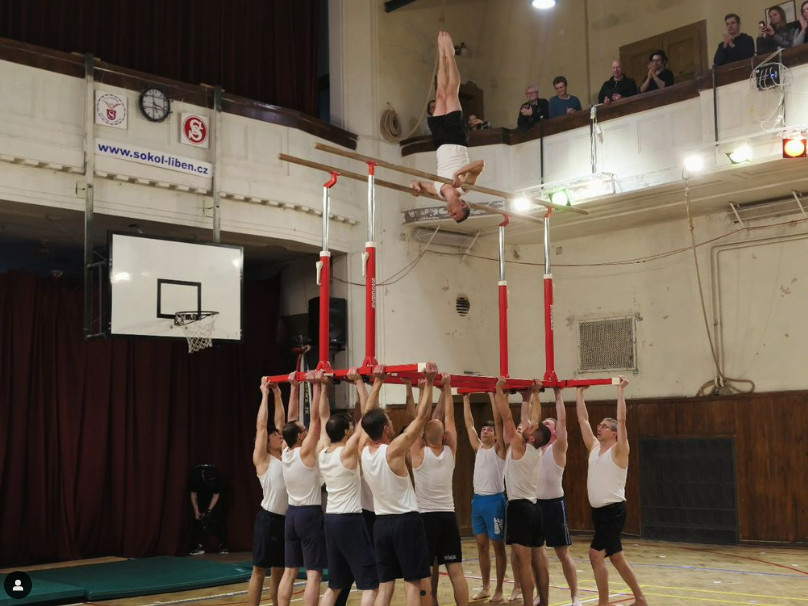
\includegraphics[width=0.8\linewidth]{./muzi_akademie.jpg}
\end{center}

Náš oddíl vešel poměrně ve známost a sem tam si poslechnem příznivé slovo nebo poděkování za inspiraci. Dokonce byl náš oddíl oceněn Sokolem roku 2019 v~kategorii kolektiv.

Letošním lednem jsme završili 10 let fungování oddílu bez vynechání jediného úterý. A~protože letos zároveň slavíme 140 let od založení jednoty, chce to uspořádat oslavu.

Mezi prapory pro jednotlivé složky v~naší sokolovně chybí prapor mužský.

Proto jsme se dohodli s~firmou Umělecké vyšívání L\&{}L Strachotovy, které šijí prapory, na podobě mužského praporu, který na podzimní slavnostní Akademii jako oddíl předáme jednotě.

\begin{wrapfigure}{l}{0.4\textwidth}
  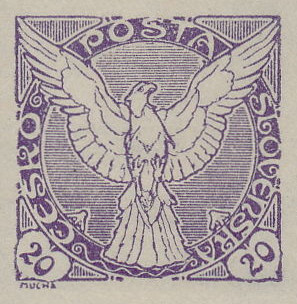
\includegraphics[width=0.9\linewidth]{./muzi_znamka.jpg}
\end{wrapfigure}

Prapor bude tmavě modrý, v~modré, jakou má klín české státní vlajky nebo i sokolské šponovky. Bílou nití na něm bude vyšit sokol z~poštovní známky Alfonse Muchy. Jednotlivé strany čtverce praporu budou lemovat čtyři antické ctnosti, tedy Moudrost – Statečnost – Uměřenost – Spravedlnost. Druhá strana bude vyšita sokolským logem v~provedení, které bude odpovídat Muchovu sokolu na druhé straně. Pod ním bude nápis Muži Sokola Libeň.

Vyšívačky Strachotovy se na náš prapor těší, sledují náš oddíl na instagramu a velice nám fandí. Bude to jejich první práce po tom, co skončí veliký nával praporů a stuh pro XVII. všesokolský slet.

\begin{wrapfigure}{r}{0.4\textwidth}
  \vspace*{-\baselineskip}
  
\includegraphics[width=\linewidth]{./QR-prapor-muzi.png}
\end{wrapfigure}

Podařilo se nám získat na prapor grant od České obce sokolské, který pokryje přibližně čtvrtinu ceny praporu, na ten zbytek bych vás nyní rád požádal o~příspěvek.

Na prapor můžete přispět libovolnou částkou na účet 107-9931340207/0100 s~variabilním symbolem 101010. Pokud budete chtít, můžeme vám na váš dar vystavit potvrzení o~daru pro vaše daňové přiznání. Peníze, které bychom vybrali navíc, použijeme k~opravám a chodu sokolovny.

Děkuji vám za vaši štědrost a těším se na dalších 10 let oddílu mužů.

\signature{Josef Kubišta}

\vspace*{24pt}

\post{Sokolská kapka krve}
Sokolové se již několik let snaží podporovat dárcovství krve a jít sami příkladem např. také projektem Sokolská kapka krve.

Veškeré informace o~projektu najdete na sokolskakapkakrve.cz. Bližší informace také rád sdělím osobně či na e-mailu: vit.jakoubek@sokol-liben.cz.

Kdo jste v~Sokole Libeň krev v~1. pololetí roku 2024 darovali, zašlete mi prosím počet odběrů na výše uvedený e-mail do 31. 7. 2024.

\signature{Vít Jakoubek}{koordinátor projektu}


\clearpage
\post{Předškolní děti}
Školní rok pomalu končí a některé děti už příští rok budou muset přejít do oddílu mladších žákyň a mladších žáků. Vzhledem k~tomu, že letos běží intenzivní nácvik na slet, není možné si vyzkoušet hodiny mladšího žactva už v~červnu. Pevně věříme, že děti přechod bez problému zvládnou.

Hodiny ve školním roce 2024/25 budou opět ve stejném čase:

\vspace*{6pt}
pondělí 16:00–17:00
čtvrtek 16:00–17:00
\vspace*{6pt}

Kdo povede které hodiny, se dozvíte na konci srpna, protože máme v~týmu dva velké \luv{}problémy\ruv{} – těhotenství a stáří.
Pokud je tedy mezi rodiči či prarodiči zájemce, který by chtěl v~oddíle předškolních dětí aktivně pomáhat, neváhejte se obrátit na vedoucí oddílu.

Kdo si místo v~oddílu předškolních dětí nerezervoval včas, riskuje, že nebude mít místo od září.

Poslední cvičení bude 17. 6. a 20. 6.

\subpost{Slet 2024}
Když jsem loni touto dobou zjišťovala, jaký bude zájem o~slet, vypadalo to, že dáme dohromady maximálně 3 celky. Nyní víme, že bude v~Edenu cvičit 5 celků, tedy 40 předškoláků / mladších školáků ve skladbě Mravenci, což je největší počet z~celé České republiky.

Držte nám palce, aby každý mravenec našel na tom velkém stadionu v~Edenu svoji značku.


Přeji pohodové prázdniny 


\signature{Dana Cejpková}{tel.: 606 551 223\\e-mail: cejpkova.dana@seznam.cz}

\vspace*{24pt}

\clearpage
\post{Oddíl rodičů a dětí}
Opět už se nám blíží další školní rok. Hlásí se mnoho zájemců o~místa v~oddíle, proto kdyby měl někdo chuť otevřít další hodinu cvičení rodičů a dětí, bude tato aktivita přijata s~nadšením.

Hodiny ve školním roce 2024/25 budou opět ve stejném čase:

\vspace*{6pt}
pondělí 16:00–17:00

úterý 9:50–10:50

čtvrtek 16:00–17:00
\vspace*{6pt}

Úterní hodinu povede Jana Motlová. Jak to bude v~pondělí a čtvrtek, se dozvíte až na konci srpna, protože Dana Cejpková jde 3. 8. na operaci s~kolenem, kdy doufá, že se vše rychle zahojí a bude moci od září bez problémů fungovat.

Vzhledem k~tomu, že letošní rok je ve znamení sletu, není možné, aby si děti vyzkoušely cvičení v~oddílu předškolních dětí. Doufáme, že všichni přechod bez problémů zvládnou.

Poslední cvičení bude 17. 6., 18. 6. a 20. 6.

\subpost{Slet 2024}
Jsme rádi, že Sokol Libeň bude mít na ploše v~Edenu jeden celý celek ve skladbě Čmeláčci. Jejich vystoupení můžete sledovat dne 5. 7., buď přímo z~tribun v~Edenu, protože některé lístky jsou ještě k~dostání, nebo v~České televizi.
V~Praze bude mnoho doprovodných programů, na které jste zváni a kterých se můžete účastnit, když na slet nenacvičujete. Všechny informace najdete na tomto webu: www.slet2024.cz.

Všem nacvičujícím bychom chtěli poděkovat, že do toho jdou, protože víme, že není úplně jednoduché dětem v~batolecím věku vysvětlit, že teď je potřeba opravdu cvičit dle pokynů.

Velký dík patří i Martině Škochové, která se do nácviku neohroženě pustila a její popisná videa s~\luv{}elektronickou tužkou\ruv{} budou rozhodně nezapomenutelná a budou inspirující pro cvičitelku, která nácvik povede za 6 let.

Přejeme krásné prázdniny

\signature{Jana, Dana a Jana}{cvičitelky rodičů a dětí}

\clearpage

\post{Thomayerovy sady}
Chcete už předem vidět, jak vypadá nácvik na slet 2024? Stačí se projít do Thomayerových sadů ke studánce, kde jsou v~trávě sletové značky. 

Zároveň bychom vás chtěli požádat, abyste při svých návštěvách parku zkontrolovali, že jsou značky na svém místě.
Pokud byste viděli, že někdo značky vyndává ze země, upozorněte ho, proč tam značky jsou a k~čemu slouží. Bohužel jsme již o~80 značek přišli.

Moc děkujeme za pomoc při dohledu nad značkami. Pokud zjistíte, že došlo k~zmizení značek, pošlete SMS na číslo: 606 551 223.

\vspace*{\baselineskip}

\begin{center}
  \includegraphics*[width=\textwidth]{thomayerovy-sady.jpg}
\end{center}

\clearpage
\post{Zdravotnické okénko}
\vspace*{-24pt}
\subpost{Zdravotní pokyny pro účastníky sletu}

Důkladně zvažte účast na sletu jako cvičenec, pokud trpíte chronickým onemocněním (ischemická choroba srdeční, hypertenze, cukrovka atd.)

Noste s~sebou platný průkaz zdravotní pojišťovny: dospělí u~sebe, u~dětí je většinou shromažďuje cvičitel.

Nezapomeňte na láhev na nápoje, pokrývku hlavy a na prostředky na ochranu proti slunci – krém na opalování s~odpovídajícím UV faktorem, sluneční brýle.
Oblečení a obuv zvolte podle předpokládaného počasí (počítejte s~možností náhlých změn), pamatujte na ochranu před úpalem a úžehem.

Vyvarujte se neznámých nebo vzhledem k~letnímu období nevhodných jídel (zmrzliny, nedopečených kuřat, majonézy) a nápojů. Dbejte na řádný pitný režim! Účastníci trpící potravinovou alergií by neměli zkoušet pokrmy, které jsou pro ně nové.

\subpost{Co se v~aplikaci Záchranka změnilo a co nás čeká?}
Důležitou změnou, která proběhla v~loňském roce, je způsob použití nouzového tlačítka. Dříve bylo potřeba tlačítko tři vteřiny podržet, nyní na něj stačí kliknout a aplikace nabídne dvě možnosti – \luv{}Zrušit aktivaci\ruv{} a \luv{}Přivolat pomoc\ruv{}\kern-0.2em. Dál všechno probíhá tak, jak jste byli zvyklí – odesílá se nouzová zpráva, aplikace předvolí linku 155, vy potvrdíte hovor a spojíte se s~operačním střediskem.

Na konci roku 2023 se podařilo v~aplikaci Záchranka spustit novou lavinovou předpověď, která je nyní vyobrazena pomocí mezinárodních piktogramů. Ty ukazují nejen stupeň nebezpečí, ale i druhy lavinových problémů a nebezpečí. Celá předpověď je doplněna o~kompletní komentář horské služby. Dostupná je pro Česko, Slovensko a Rakousko. Oblasti se rozšiřují o~Slovinsko, Itálii, Německo, Rumunsko a Španělsko – přivolání pomoci včetně odeslání polohy a dat se v~těchto zemích plánuje. Aktuálně vás v~těchto místech aplikace pouze přepojí na místní tísňovou linku.

V~Jihomoravském kraji se nově spouští také spolupráce s~dálniční policií Jihomoravského kraje. V~praxi to znamená, že pokud si ve kterékoliv části dálnice v~kraji přivoláte pomoc z~aplikace Záchranka, informace o~poloze dostane nejen ZZS Jihomoravského kraje, ale také dispečink dálniční policie. Bude tak pro ně mnohem rychlejší a jednodušší nehodu najít  a vyřešit.

\signature{Vít Jakoubek}{zdravotník jednoty}
\vspace*{24pt}

\post{Sportovní medicína ustupuje od ledování}
Led se běžně doporučuje jako první pomoc při poranění měkkých tkání~– podvrtnutí kloubů a poranění vazivového aparátu, zhmoždění či natržení svalů a šlach nebo po operačních zákrocích. V~současné době se zejména ve sportovní medicíně od použití ledu postupně upouští, a to především z~důvodu prodloužení hojení takto poraněného místa.

\begin{center}
  \textbf{Historie ledování}
\end{center}

Ledování se začalo v~medicíně využívat ve 40. letech 20. století k~redukci krevních ztrát, bolesti a zánětu. V~roce 1978 přišel dr. Gabe Mirkin s~doporučeným postupem po úrazech měkkých tkání se zkratkou RICE (rest, ice, compression a elevation), tedy klid, led, komprese a elevace. Později se zkratka rozšířila o~P (protection = ochrana), tedy na zkratku PRICE. V~roce 2013 začal sám dr. Mirkin využití ledu zpochybňovat a potvrzují to i vědecké studie, které se v~posledních letech tématem zabývají.


\begin{center}
  \textbf{Proč neledovat?}
\end{center}

Led má nezpochybnitelný účinek ve snižování bolesti, snížení krevního průtoku a vzniku otoku. Cílená kryoterapie také snižuje lokálně zánětlivou reakci těla, ta je ale právě důležitou součástí hojivého procesu. Bez zánětu nedojde k~nastartování  opravy a přestavby poraněné tkáně a omezuje se přísun bílých krvinek do místa poškození. V~roce 2011 proběhla studie sledující hojení svalových zranění u~sportovců, kdy jedna skupina z~nich led použila a druhá ne. Po prvních dnech od úrazu se u~skupiny, která neledovala, objevilo větší množství makrofágů – tedy buněk imunitního systému. Po 28 dnech od úrazu byla regenerace svalu u~této skupiny o~65\% větší a zároveň tkáň obsahovala méně jizev. To dokazuje zkrácení času rekonvalescence a zvýšení efektivity hojení při vynechání chladové terapie.

Tlumení zánětu je tedy nežádoucím účinkem ledování. Zbývá snižování bolesti a otoku. Edém je při hojení nevítaný, pro jeho redukci je ale vhodnější využití komprese a elevace (zvednutí poškozeného místa) a izometrické cvičení. Kontrakcí okolních svalů lze dosáhnou efektu pumpy a tím pomoci v~odplavení metabolitů z~místa poškození. Redukce bolesti a současně placebo efekt může být skutečným přínosem ledování. Převyšuje tento benefit ostatní negativa? 


\begin{center}
  \textbf{Jak tedy postupovat po úrazu}
\end{center}

V~první řadě je potřeba vyloučit závažné poranění, jako jsou zlomeniny či výraznější poškození vazivového nebo svalového aparátu. Proto je vhodné u~závažnějšího poranění navštívit lékaře. Další postup se řídí novou zkratkou \textit{PEACE and LOVE}, kterou si níže vysvětlíme.

\vspace*{6pt}

\textit{P = Protection} – ochrana poraněného místa před dalším poškozením. U~podvrtnutého kotníku to mohou být například berle a tím odlehčení končetiny, případně ortéza.

\textit{E = Elevation} – zvednutí poraněné končetiny.

\textit{A~= Avoid anti-inflammatories} – vyloučení protizánětlivých léků. Jak již bylo řečeno, zánět je nedílnou součástí hojivého procesu. Pokud je potřeba použít lék proti bolesti, je lepší zvolit například Paralen, který nemá protizánětlivé účinky.

\textit{C = Compression} – komprese postiženého místa například pružným obinadlem. To je nejúčinnější metoda pro redukci otoku a hematomu, což je vhodné co nejdříve po vzniku úrazu. 

\textit{E = Education} – edukace zraněného, jaká opatření využít. Tento bod lze také chápat jako naslouchání vlastního těla, respektování bolesti či konzultaci s~odborníkem.

%\vspace*{6pt}

Tyto body se vztahují k~prvním dnům po zranění. Následně se postupuje podle druhé zkratky LOVE, která je vhodná v~dalších dnech až týdnech, tedy po odeznění akutních příznaků.

\vspace*{6pt}

\textit{L = Load} – postupné zvyšování zátěže a návrat k~normálnímu pohybu. Intenzitu zátěže lze určit podle bolesti.

\textit{O~= Optimism} – sebejistota a důvěra ve vlastní tělo vede k~rychlejšímu zotavení. Podstatný vliv na rekonvalescenci má totiž psychika.

\textit{V~= Vascularisation} – novotvorba cév a prokrvení. Vhodná aktivita nezpůsobující bolest a aktivace svalů v~okolí poraněného místa pomáhají prorůstání tkáně novými cévami. 

\textit{E = Exercise} – posilovací, protahovací a balanční cvičení mají v~následné rehabilitaci větší význam pro plné zotavení než dlouhodobý klid. Dochází během něj k~obnově síly, mobility a propriocepce.

\vspace*{6pt}

Uvedený postup tedy zcela vynechává jakékoli využití chladu. Ledování stále může mít svůj přínos ve specifických případech, například pokud je nutná výraznější redukce otoku před operací poraněného místa. Pro léčbu méně závažných poranění měkkých tkání ale převládají spíše jeho nevýhody.

\signature{Michal Přibyl}{}

% zadní obálka
\clearpage

\pagestyle{blank}
\newgeometry{margin=1cm}

\vspace*{96pt}

\pagecolor{sokolred}
\color{white}

\noindent {\fontsize{48pt}{56pt}\tyrs
se sokolským

\vspace*{24pt}

\noindent nazdar!}

\vspace*{\fill}

% \color{black}
\begin{center}
Vydává Tělocvičná jednota Sokol Libeň, Zenklova 37, Praha 8

\vspace*{12pt}

Na přípravě tohoto čísla se spolu s~autory jednotlivých textů podíleli:

grafická úprava – Martin Burian | jazyková úprava – Martina Waclawičová \\ editoři textů – Vít Jakoubek, Jan Přech
\end{center}

\end{document}